% !TEX encoding = UTF-8
% !TEX program = pdflatex
% !TEX root = relazione.tex
% !TeX spellcheck = it_IT

% ESEMPI
\section{Esempi}\label{sec:esempi}
Verranno presentati ora alcuni esempi di utilizzo delle API con l'obbiettivo di eseguire un confronto il più imparziale possibile.
Sono state quindi individuate alcune funzionalità comuni a tutte le piattaforme: riconoscimento oggetti e ambientazione, riconoscimento di volti (singolo e con più volti).
%%
\subsection{Riconoscimento oggetti e ambientazione}\label{subsec:riconscimento-oggetti-ambientazione}
Data l'immagine in Figura~\ref{fig:riconscimento-oggetti-ambientazione}, dopo aver interrogato le relative API per il riconscimento di oggetti/tagging,
i risultati sono stati riassunti in Tabella~\ref{tab:riconscimento-oggetti-ambientazione}; in questa si possono osservare le categorie o etichette sotto le quali
gli oggetti sono stati identificati e il loro livello di affidabilità.
Inoltre, utilizzando le API di Microsoft C.S. è stata generata anche una descrizione.
%
\begin{figure}[!h]
\begin{center}
	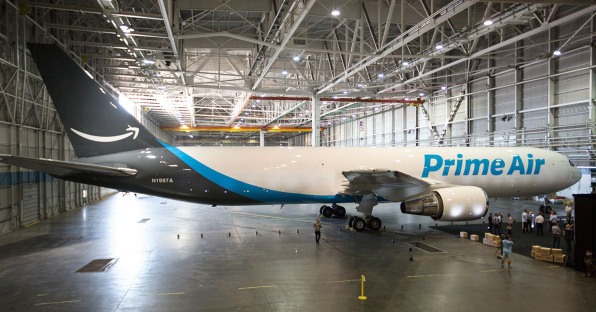
\includegraphics[width=.6\paperwidth]{prime-air.jpg}
{\scriptsize \caption{Immagine utilizzata come riferimento in questo confronto.}
\label{fig:riconscimento-oggetti-ambientazione}}
\end{center}
\end{figure}
%
\begin{table}[!h]
\centering
{\footnotesize
\resizebox{\textwidth}{!}{
\begin{tabularx}{\textwidth}{c?l|l|l|l}
\toprule
						& Microsoft C.S   & IBM W.S.       & Amazon A. I. & Google C.M.L.S. \\ \hline
\midrule
Etichette   			& plane (97,41\%)                & hangar (97,9\%)           & Hangar (95,74\%)               & Airliner (96\%)             \\
& indoor (96,20\%)               & blue color (85,9\%)       & Aircraft (89,96\%)             & Airline (95\%)              \\
& floor (96,10\%)                & steel blue color (75,5\%) & Airplane (89,96\%)             & Airplane (95\%)             \\
& airplane (91,19\%)             &                           & Warplane (66,30\%)             & Vehicle (91\%)              \\
& airport (91,11\%)              &                           & Jet (57,09\%)                  & Air travel (90\%)           \\
& aircraft (72,66\%)             &                           & Landing (52,80\%)              & Aircraft (87\%)             \\
& transport (67,56\%)            &                           &                                & Aviation 85\%)              \\	\hline
Descrizione & a large airplane at an airport & -                         & -                              & -				\\
\bottomrule
\end{tabularx}}
\caption{Tabella riassuntiva per il riconscimento oggetti e ambientazione.}
\label{tab:riconscimento-oggetti-ambientazione}}
\end{table}
%%
\subsection{Riconoscimento di un volto}\label{subsec:riconscimento-singolo-volto}
In questo confronto lo scopo era quello di verificare le caratteristiche del volto (\textit{landmark}) che l'API era in grado di riconsoscere in un ambiente semplice;
per questo motivo è stata scelta un'immagine di un primo piano di una ragazza\footnote{I diritti dell'immagine sono dei rispettivi proprietari.}.
Come si può notare dai risultati in Figura~\ref{fig:riconscimento-singolo-volto}, tutte le API hanno riconosciuto e identificato correttamente il volto e, a parte
il servizio offerto da IBM, diversi elementi di questo.
Il migliore di questi sembrerebbe essere le API di Google che, tuttavia, non fornisce indicazioni sulla persona specifica (età, sesso).
\begin{figure}[!h]
\begin{center}
	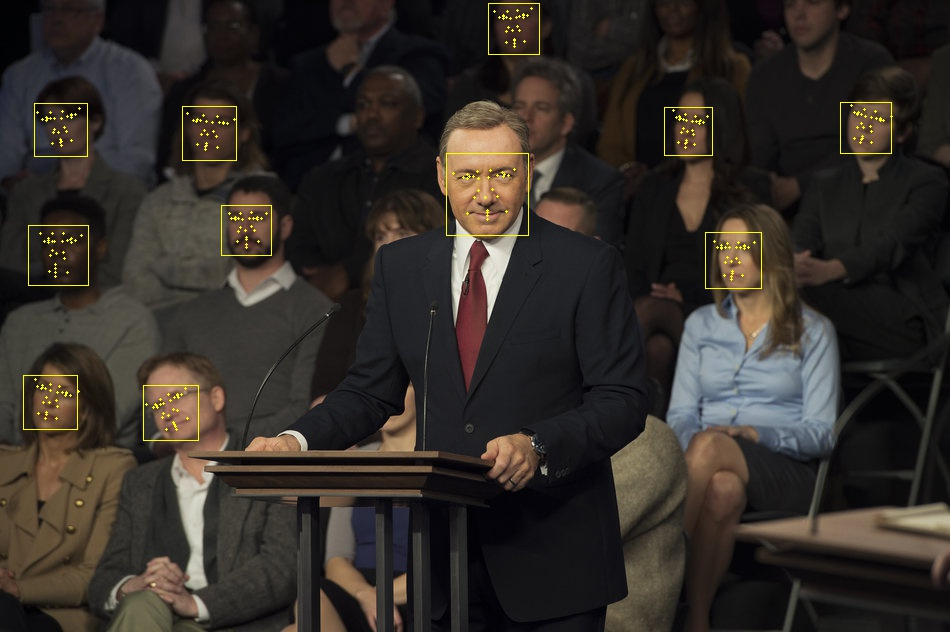
\includegraphics[width=200px,height=282px]{riconoscimento-viso-1/microsoft.jpg}
	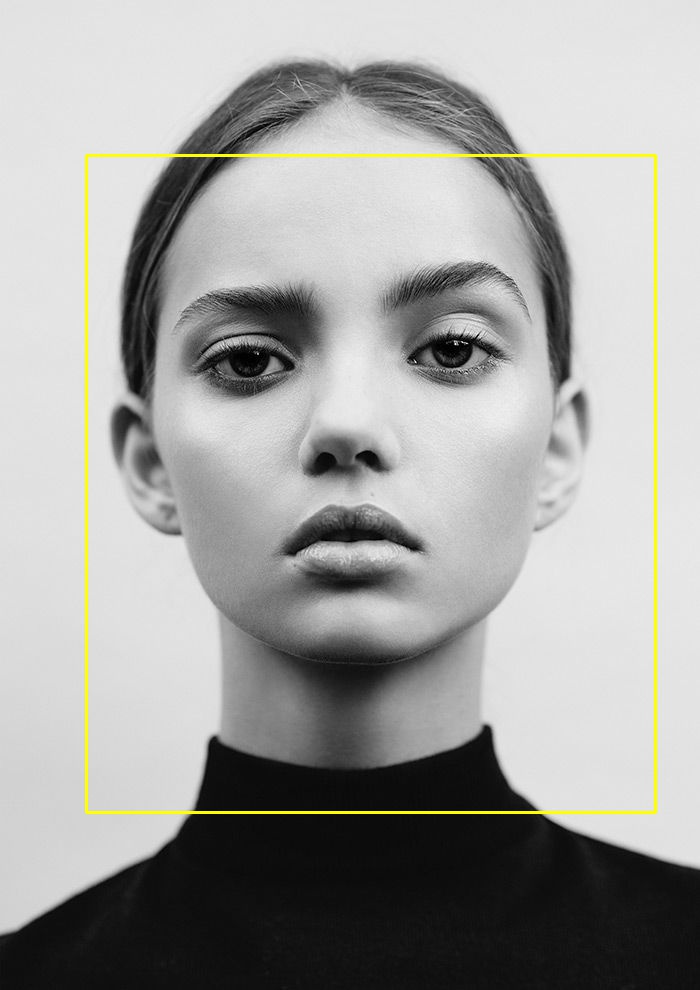
\includegraphics[width=200px,height=282px]{riconoscimento-viso-1/ibm.jpg}
	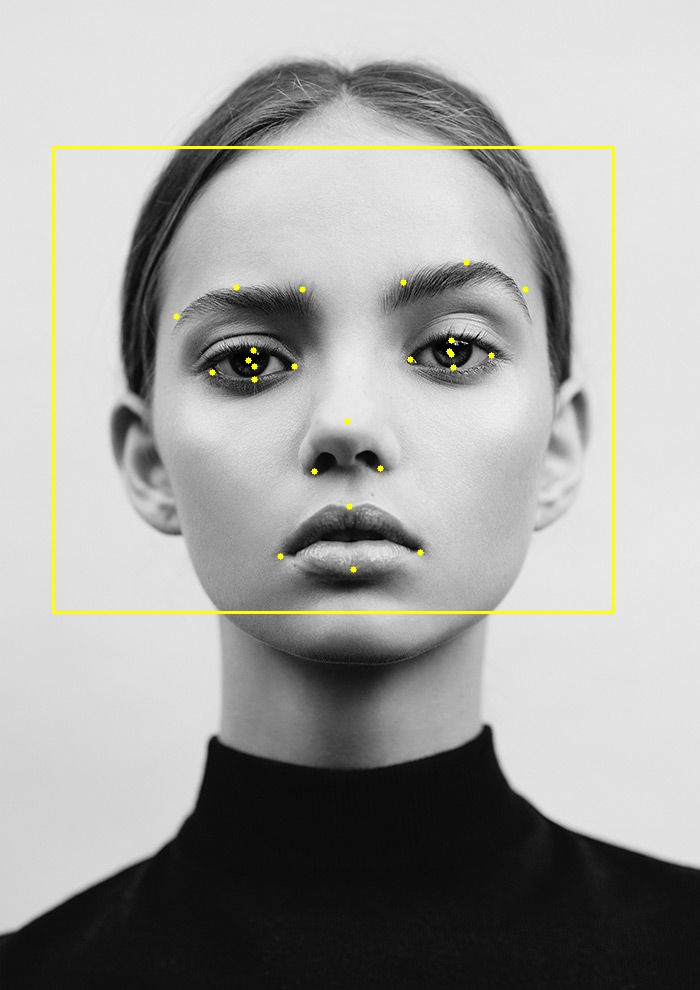
\includegraphics[width=200px,height=282px]{riconoscimento-viso-1/amazon.jpg}
	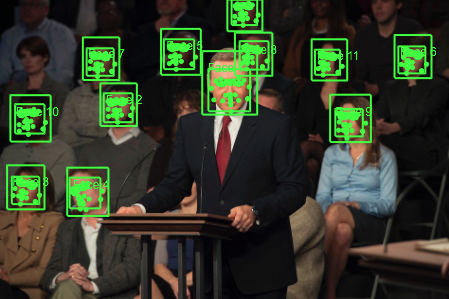
\includegraphics[width=200px,height=282px]{riconoscimento-viso-1/google.png}
{\scriptsize \caption{Riconscimento di un singolo volto utilizzando le API di (da sinistra): Microsoft, IBM, Amazon, Google. (Fonte: \url{http://eddienew.com})}
\label{fig:riconscimento-singolo-volto}}
\end{center}
\end{figure}
%
\subsection{Riconoscimento di più volti}\label{subsec:riconscimento-piu-volti}
%
